\documentclass[tikz]{standalone}
\usetikzlibrary{patterns}
\usetikzlibrary{shapes,arrows}
\usetikzlibrary{decorations.pathreplacing, positioning}
\definecolor{greengreen}{rgb}{0.0, 0.42, 0.24}
\definecolor{calpolypomonagreen}{rgb}{0.12, 0.3, 0.17}
\definecolor{forestgreen}{rgb}{0.13, 0.55, 0.13}

\begin{document}
\noindent
  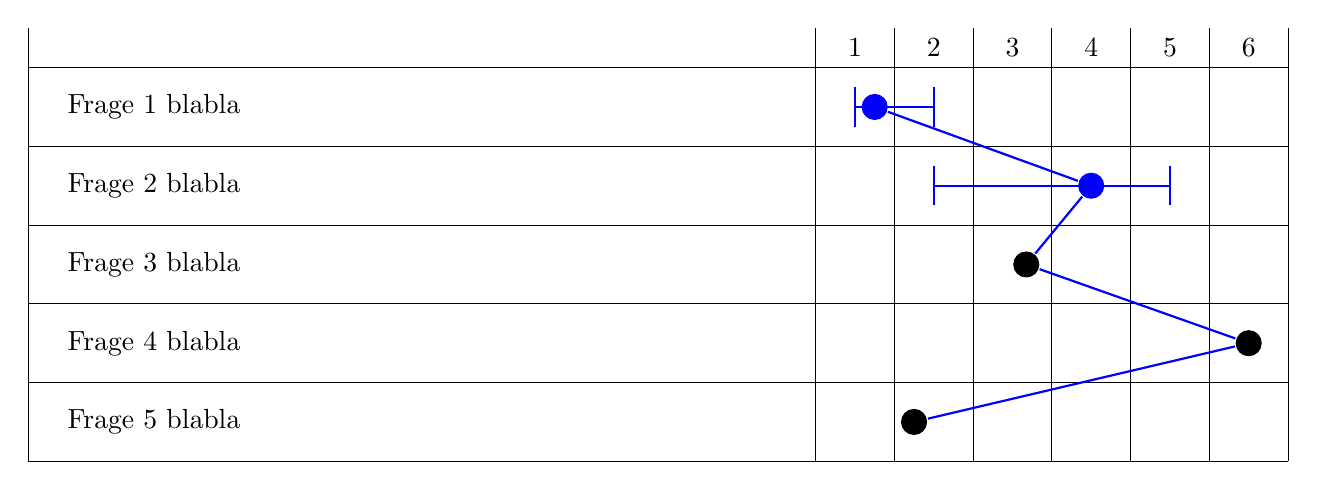
\begin{tikzpicture}

    \foreach \y in {0,1,2,3,4,5}
        \draw (0, 0 - \y) -- (16, 0 - \y);
    \foreach \x in {0,10,11,12,13,14,15,16}
        \draw (0 + \x, 0.5) -- (0 + \x, - 5);
    
    \node at (10.5, 0.25) {$1$};
    \node at (11.5, 0.25) {$2$};
    \node at (12.5, 0.25) {$3$};
    \node at (13.5, 0.25) {$4$};
    \node at (14.5, 0.25) {$5$};
    \node at (15.5, 0.25) {$6$};

    \node[thick,  align=left, text width=9cm] at (5, -0.5) {Frage 1 blabla};
    \node[thick,  align=left, text width=9cm] at (5, -1.5) {Frage 2 blabla};
    \node[thick,  align=left, text width=9cm] at (5, -2.5) {Frage 3 blabla};
    \node[thick,  align=left, text width=9cm] at (5, -3.5) {Frage 4 blabla};
    \node[thick,  align=left, text width=9cm] at (5, -4.5) {Frage 5 blabla};

    
    \draw[blue,thick] (10.5, -0.25) -- (10.5, -0.75);
    \draw[blue,thick] (11.5, -0.25) -- (11.5, -0.75);
    \draw[blue,thick] (10.5, -0.5) -- (11.5, -0.5);
    \node[thick, circle, fill=blue, minimum width=0.25] (1) at (10.75, -0.5) {};

    \draw[blue,thick] (11.5, -1.25) -- (11.5, -1.75);
    \draw[blue,thick] (14.5, -1.25) -- (14.5, -1.75);
    \draw[blue,thick] (11.5, -1.5) -- (14.5, -1.5);
    \node[thick, circle, fill=blue, minimum width=0.25] (2) at (13.5, -1.5) {};

    \node[thick, circle, fill=black, minimum width=0.25] (3) at (12.675, -2.5) {};
    \node[thick, circle, fill=black, minimum width=0.25] (4) at (15.5, -3.5) {};
    \node[thick, circle, fill=black, minimum width=0.25] (5) at (11.25, -4.5) {};

    \draw[color=blue, thick] (1) to (2) to (3) to (4) to (5);

  \end{tikzpicture}%
\end{document}
